% Indicate the main file. Must go at the beginning of the file.
% !TEX root = ../main.tex

%%%%%%%%%%%%%%%%%%%%%%%%%%%%%%%%%%%%%%%%%%%%%%%%%%%%%%%%%%%%%%%%%%%%%%%%%%%%%%%%
% 03_results
%%%%%%%%%%%%%%%%%%%%%%%%%%%%%%%%%%%%%%%%%%%%%%%%%%%%%%%%%%%%%%%%%%%%%%%%%%%%%%%%

\section{Results}
\label{results}

The best-performing model achieved an accuracy of 0.9274 and a weighted F1 Score of 0.9275.
The results for all trained models are summarized in \autoref{tab:accuracy_f1_table}.
All trained models for the simplified perviousness lead the ranking, followed by the
models for the perviousness classification and the category classification
with accuracies of around 0.88 and 0.59, respectively. Only the label type \texttt{sealed\_simple}
will be considered for further analysis, as it is the most relevant for the study area.

\begin{table}[H]
    \centering
    \caption{Accuracy and F1 Score for all trained models, arranged by accuracy.}
    \small
    \label{tab:accuracy_f1_table}
    \begin{tabular}{llllll}
    \toprule
    LabelType & Augmented & LearningRate & WeightDecay & Accuracy & F1 Score \\
    \midrule
    sealed\_simple  & True      & 0.0001    & 0.1   & 0.9274    & 0.9275 \\
    sealed\_simple  & False     & 0.0001    & 0.01  & 0.9109    & 0.9112 \\
    sealed\_simple  & True      & 0.001     & 0.1   & 0.9069    & 0.9072 \\
    sealed\_simple  & True      & 0.0001    & 0.01  & 0.9034    & 0.9038 \\
    sealed\_simple  & True      & 0.001     & 0     & 0.9028    & 0.9032 \\
    sealed\_simple  & False     & 0.001     & 0.1   & 0.9021    & 0.9024 \\
    sealed\_simple  & True      & 0.0001    & 0     & 0.9007    & 0.9011 \\
    sealed\_simple  & False     & 0.0001    & 0.1   & 0.9000    & 0.9004 \\
    sealed\_simple  & False     & 0.001     & 0.01  & 0.8999    & 0.9001 \\
    sealed\_simple  & False     & 0.001     & 0     & 0.8996    & 0.9000 \\
    sealed\_simple  & True      & 0.001     & 0.01  & 0.8980    & 0.8984 \\
    sealed\_simple  & False     & 0.0001    & 0     & 0.8977    & 0.8980 \\
    sealed          & False     & 0.001     & 0.01  & 0.8817    & 0.8716 \\
    sealed          & True      & 0.001     & 0.01  & 0.8763    & 0.8619 \\
    category        & True      & 0.001     & 0.01  & 0.5902    & 0.5722 \\
    category        & False     & 0.001     & 0.01  & 0.5806    & 0.5665 \\
    \bottomrule
    \end{tabular}
\end{table}

\subsection{Hyperparameter Tuning}%%%%%%%%%%%%%%%%%%%%%%%%%%%%%%%%%%%%%%%%%%%%%%

The hyperparameter tuning results included in \autoref{tab:accuracy_f1_table} and
visualized in \autoref{fig:hp_tuning_boxplot} show that the \texttt{learning\_rate} of 0.0001
performs better and that a \texttt{weight\_decay} of 0.1 leads to the best results when
combined with data augmentation. Overall, data augmentation seems to have a positive
effect on accuracy, but there is an exception for \texttt{weight\_decay} of 0.01,
where the accuracy is higher without data augmentation.

\begin{figure}[H]
    \centering
    \captionsetup{width=0.8\linewidth}
    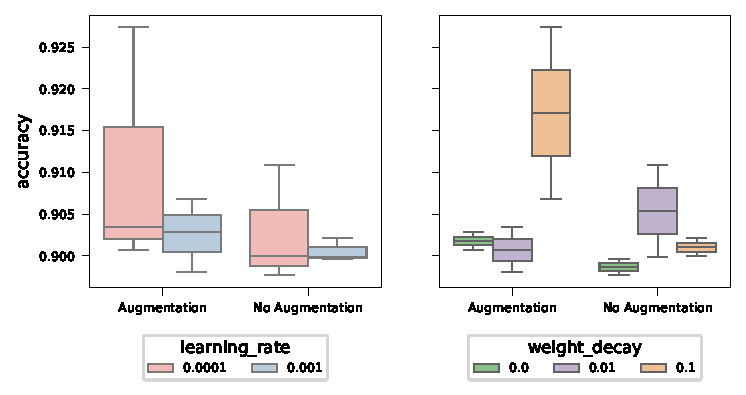
\includegraphics{figures/hp_tuning_boxplot.pdf}
    \caption{Accuracy of the models for the different hyperparameters grouped by use of data augmentation.}
    \label{fig:hp_tuning_boxplot}
\end{figure}

\subsection{Best Model}%%%%%%%%%%%%%%%%%%%%%%%%%%%%%%%%%%%%%%%%%%%%%%%%%%%%%%%%%

The best-performing model was the one for the simplified perviousness classification
with the following hyperparameters:
\begin{itemize}
    \item Learning rate: 0.001
    \item Weight decay: 0.01
    \item Data augmentation applied
\end{itemize}
It achieved an accuracy of 0.927 and a weighted F1 Score of 0.927.
The F1 Score per class was 0.92 for class \texttt{'unsealed'} and 0.93 for class \texttt{'sealed'}.
For a visual inspection of the predictions, refer to \autoref{fig:best_model_visual}.
The accuracy per category, shown in \autoref{fig:best_model_accuracy_per_category}, shows categories
like \texttt{Building}, \texttt{BuildingDistortion} and \texttt{GreenArea} predicted with an accuracy between 0.8 and 0.9.
The categories \texttt{RoadAsphalt}, \texttt{Forrest} and \texttt{MeadowPasture} where predicted with an accuracy above 0.95.
The categories \texttt{ConstructionSite}, \texttt{WaterBasin}, \texttt{Path} and \texttt{SealedObjects} where predicted with
an accuracy below 0.8. To investigate the incorrect predictions further, a plot was created that shows the incorrectly
predicted pixels colored by land cover category in \autoref{fig:incorrect_per_category}. Since in the
rural test area it was not showing much, the plot is limited to the urban and industrial test areas.

\begin{figure}[H]
    \centering
    \captionsetup{width=0.8\linewidth}
    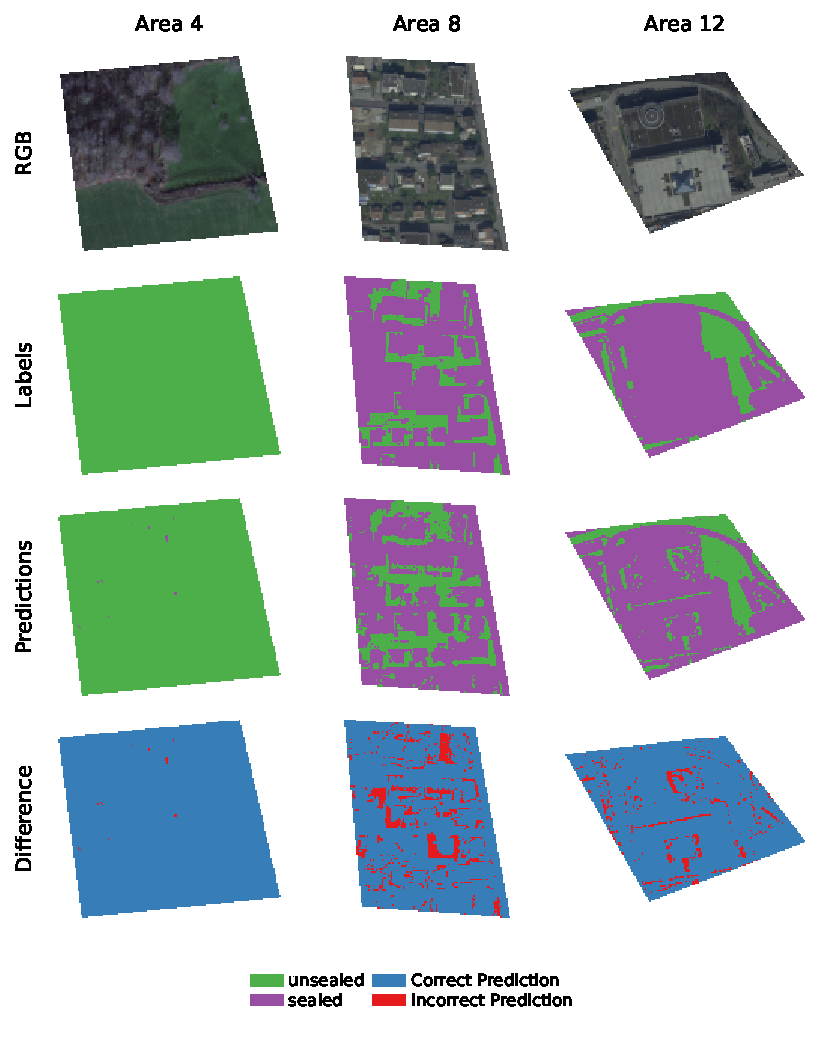
\includegraphics{figures/best_model_visual.pdf}
    \caption{Visual inspection of the predictions for the test areas of the best model.}
    \label{fig:best_model_visual}
\end{figure}

\begin{figure}[H]
    \centering
    \captionsetup{width=0.8\linewidth}
    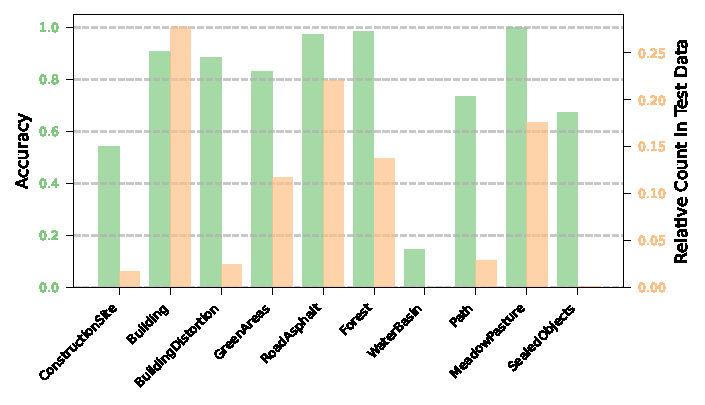
\includegraphics{figures/best_model_accuracy_per_category.pdf}
    \caption{Accuracy per category for the best-performing model including the relative count of available data for each category.}
    \label{fig:best_model_accuracy_per_category}
\end{figure}

\begin{figure}[H]
    \centering
    \captionsetup{width=0.8\linewidth}
    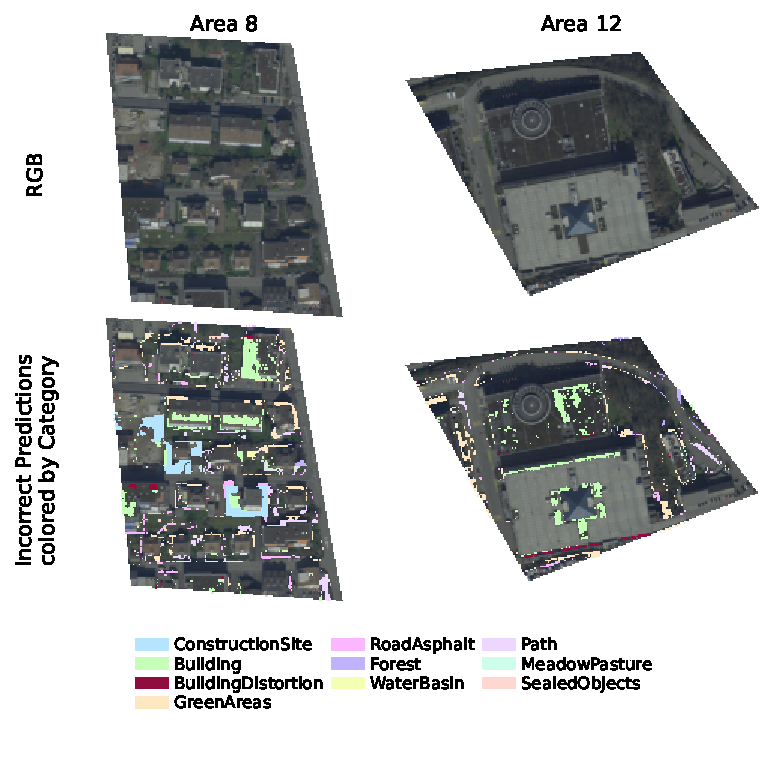
\includegraphics{figures/incorrect_per_category.pdf}
    \caption{Incorrectly predicted pixels colored by land cover category on the bottom row. The top row shows the RGB image for reference.}
    \label{fig:incorrect_per_category}
\end{figure}



